\section{User Interface}
\label{sec:user-interface}
\writer{Morten}

The following section will describe how the Graphical User Interfaces (GUIs) of the Petri net editor, Geometry editor, Appearance editor, Configuration editor and the Simulation window should look like. How to execute different tasks in the editors, such as creating and editing Geometries and Petri nets, will be described in the handbook. 

The different editors will strive towards being intuitive for the targeted user, e.g. the Geometry editor should be easy to use for the non-technical user, while the Petri net editor should be intuitive for the Petri net engineer.

\subsection{Technologies}
The editors will be implemented as extensions to Eclipse, which allows us to use the different functionalities that comes with Eclipse. The functionalities listed below are all part of Eclipse and will be used for this software.

\begin{itemize}
\item{\textbf{Editor:} Used for the Petri net editor and the Geometry editor. Gives the user the ability to create and edit Petri nets and geometries.}
\item{\textbf{View:} Used to show properties of the object selected in the editor and the project files.}
\item{\textbf{Dialog:} A pop-up window used when the user has to specify a property of an object or to select textures or 3D files in the Appearance editor.}
\item{\textbf{Wizard:} A pop-up window with several pages that guides the user to fill out information correctly. Used to set up the configuration for the simulator.}
\end{itemize}

The use of these features will be further explained in the user handbook. 

\subsection{Graphical User Interface}
This section will describe the GUI for the editors and the simulation tool. 

\subsubsection{Introduction to Petri net editor \& Geometry editor.}
The Petri net and Geometry editors are very much alike. They have the same composition and only the objects that can be drawn on the canvas are different. Both editors have from the ePNK two kinds of editors: a tree editor and a diagram editor. The diagram editor consist of a palette, a view with the project files, a view with the properties of the selected object and a canvas. The tree editor has a project explorer, properties view and a view with the tree of objects. Examples of the Petri net and Geometry editors  can be seen in figure \ref{fig:petrinet_tree} \& \ref{fig:petrinet_diagram} and figure \ref{fig:geometry_tree} \& \ref{fig:geometry_diagram} respectively. 

\begin{figure}[H]
\begin{center}
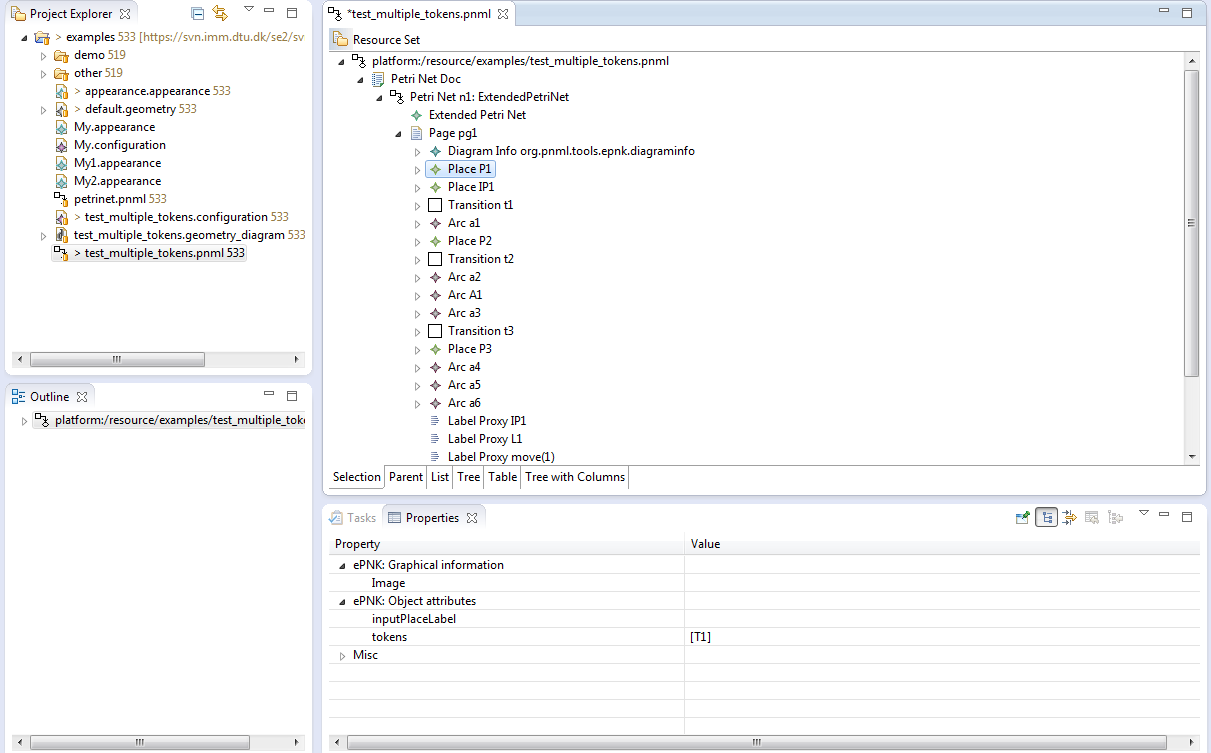
\includegraphics[scale=0.45]{image/ui/petrinet_tree.png}
\caption{The Petri net tree editor.}
\label{fig:petrinet_tree}
\end{center}
\end{figure}

\begin{figure*}[H]
\begin{center}
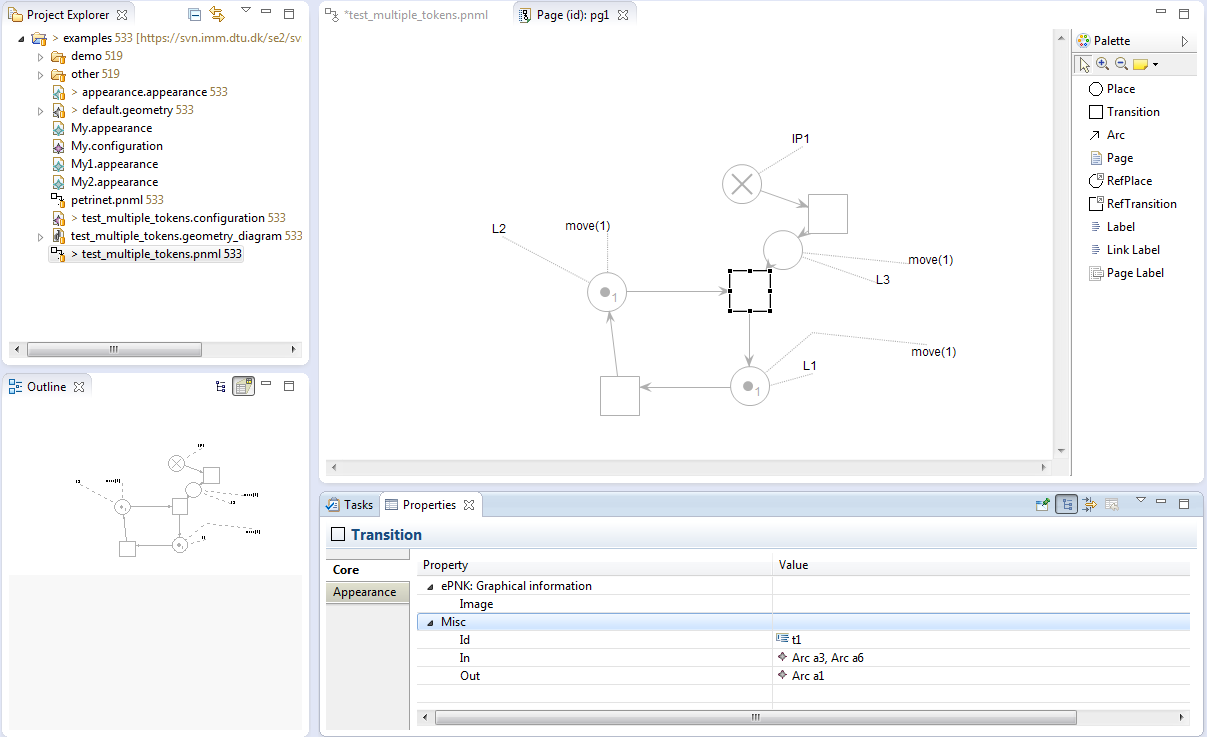
\includegraphics[scale=0.45]{image/ui/petrinet_diagram.png}
\caption{The Petri net diagram editor.}
\label{fig:petrinet_diagram}
\end{center}
\end{figure*}

\begin{figure}[H]
\begin{center}
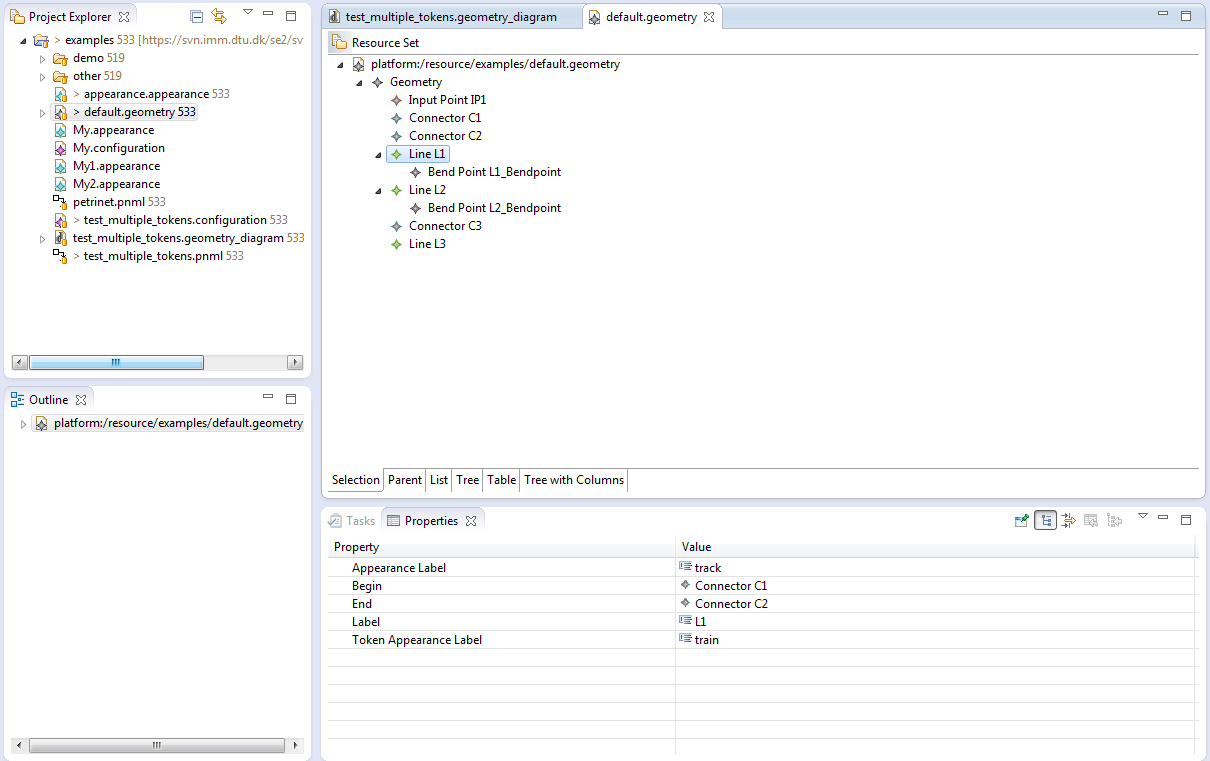
\includegraphics[scale=0.45]{image/ui/geometry_tree.png}
\caption{The geometry tree editor.}
\label{fig:geometry_tree}
\end{center}
\end{figure}

\begin{figure*}[H]
\begin{center}
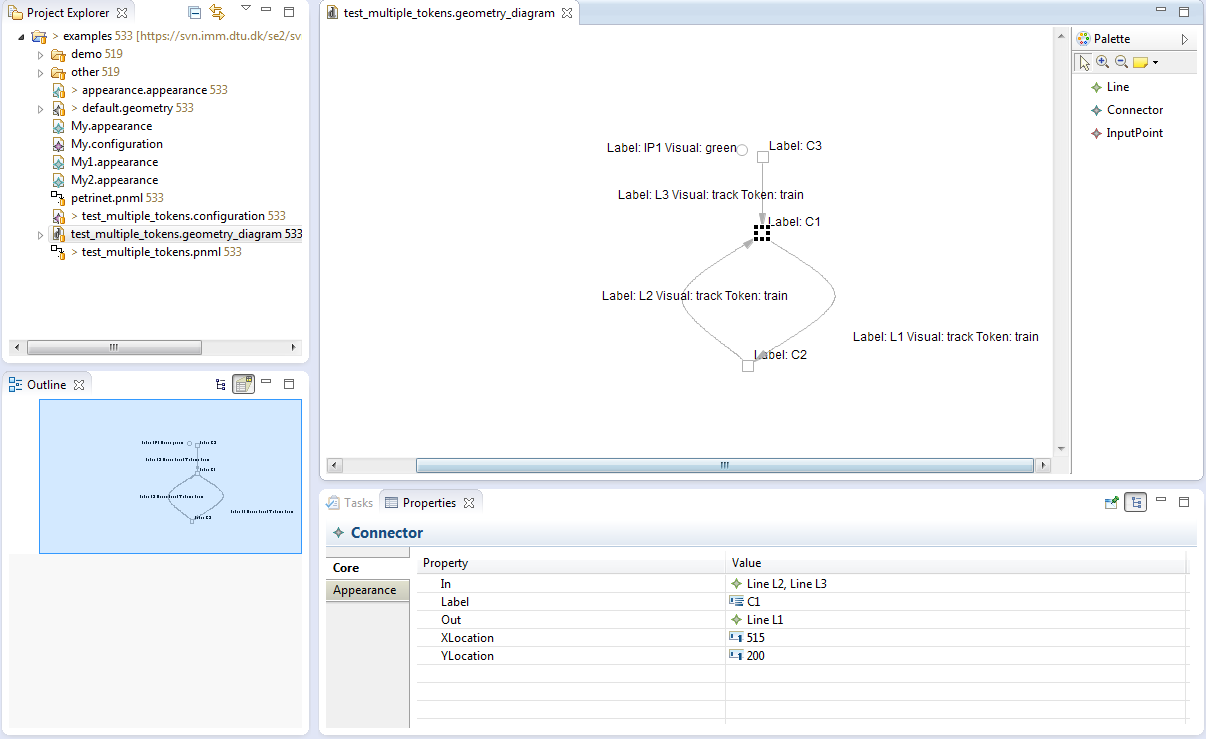
\includegraphics[scale=0.45]{image/ui/geometry_diagram.png}
\caption{The geometry diagram editor.}
\label{fig:geometry_diagram}
\end{center}
\end{figure*}

\subsubsection{Petri net editor}
\textbf{Project explorer} \\
On the left side, the user will have a view where all the files associated to the project are shown. This view will be able to identify the type of each file and, when the user opens one of the files, the editor associated to the file type will open accordingly. 

\textbf{Canvas (diagram editor)} \\
The canvas is the place where the user can create/draw the Petri net. In the diagram editor the user selects an object from the palette and left-click on the canvas to create the object. The user can edit the position of the different objects by dragging them around the canvas. Furthermore, the connections between the objects can be edited by dragging lines between two objects (while following the rules of the Petri net). The user will be able to see the graphical representation of the Petri net in the Petri net diagram editor. 

\textbf{Palette} \\
To create and modify the Petri net the user will be able to create objects on the canvas by selecting the desired tool in the palette on the right side. The palette in the Petri net editor has tools to create places, transistions and arcs. Each object will have a dedicated icon in order to increase the usability of the GUI.

\textbf{Tree editor} \\
In the tree editor the user can create objects by right-clicking and select Add object. The tree editor gives the user a quick overview of how the different objects are connected.

\textbf{Object properties} \\
Each object has different properties that can be defined by the user. The user can modify these properties in the properties view whenever an object is selected. The different objects have the properties: \\
\textbf{Transistion}
\begin{itemize}
\item{\textbf{Id:} The id of the object used in the simulator.}
\item{\textbf{In:} The incoming arcs.}
\item{\textbf{Out:} The outgoing arcs.}
\end{itemize}
\textbf{Place}%%%%%%%%%%%%
\begin{itemize}
\item{\textbf{Id:} The id of the object used in the simulator.}
\item{\textbf{In:} The incoming arcs.}
\item{\textbf{Out:} The out going arcs.}
\item{\textbf{Tokens:} A list of tokens placed on this place.}
\item{\textbf{Input place label:} Determines whether the place is an input place. Can either be true of false.}
\end{itemize}
\textbf{Arc}%%%%%%%%%%%%
\begin{itemize}
\item{\textbf{Id:} The id of the object used in the simulator.}
\item{\textbf{Source:} The source object.}
\item{\textbf{Target:} The target object.}
\end{itemize}

\subsubsection{Geometry editor}
\textbf{Project explorer} \\
On the left side, the user will have a view where all the files associated to the project are shown. This view will be able to identify the type of each file and, when the user opens one of the files, the editor associated to the file type will open accordingly. 

\textbf{Canvas (diagram editor)} \\
The canvas is the place where the user can create/draw the geometry. In the diagram editor the user selects an object from the palette and left-click on the canvas to create the object. The user can edit the position of the different objects by dragging them around the canvas. Furthermore, the connections between the objects can be edited by dragging lines between two objects. The user can create bend points on these lines to modify the slopes of the lines. The user will be able to see the graphical representation of the Petri net in the Petri net diagram editor. 

\textbf{Palette} \\
To create and modify the geometry, the user will be able to create objects on the canvas by selecting the desired tool in the palette on the right side. The palette in the geometry editor has tools to create input places, connections and lines. Each object will have a dedicated icon in order to increase the usability of the GUI.

\textbf{Object properties} \\
Each object has different properties that can be defined by the user. The user can modify these properties in the properties view whenever an object is selected. The different objects have the properties: \\
\textbf{Input place}
\begin{itemize}
\item{\textbf{Appearance label:} The appearance label is used in the appearance editor where the user specify the appearance in the 3D simulation of the specific label.}
\item{\textbf{Label:} Used in the 3D engine for recognition.}
\item{\textbf{X and Y location:} The position in the simulation.}
\end{itemize}
\textbf{Connector}
\begin{itemize}
\item{\textbf{Label:} Used in the 3D engine for recognition.}
\item{\textbf{In:} The incoming lines.}
\item{\textbf{Out:} The outgoing lines.}
\item{\textbf{X and Y location:} The position in the simulation.}
\end{itemize}
\textbf{Line}
\begin{itemize}
\item{\textbf{Appearance label:} The appearance label is used in the appearance editor where the user specify the appearance in the 3D simulation of the specific label.}
\item{\textbf{Begin:} The source connector.}
\item{\textbf{End:} The target connector.}
\item{\textbf{Label:} Used in the 3D engine for recognition.}
\item{\textbf{Token appearance label:} The appearance label of the tokens on this line. The user specifies the appearance in the appearance editor.}
\end{itemize}

\subsubsection{Appearance editor}
Figure \ref{fig:appearance_editor} is an example of the appearance editor. The user has previously specified, in the Petri net editor, the appearance labels for each object. The user creates a new Appearance object (AObject) in the editor and gives it the same label as given in the Geometry editor. The user can specify the texture and model of the appearance in the texture and Object3D property.

\begin{figure}[ht]
\begin{center}
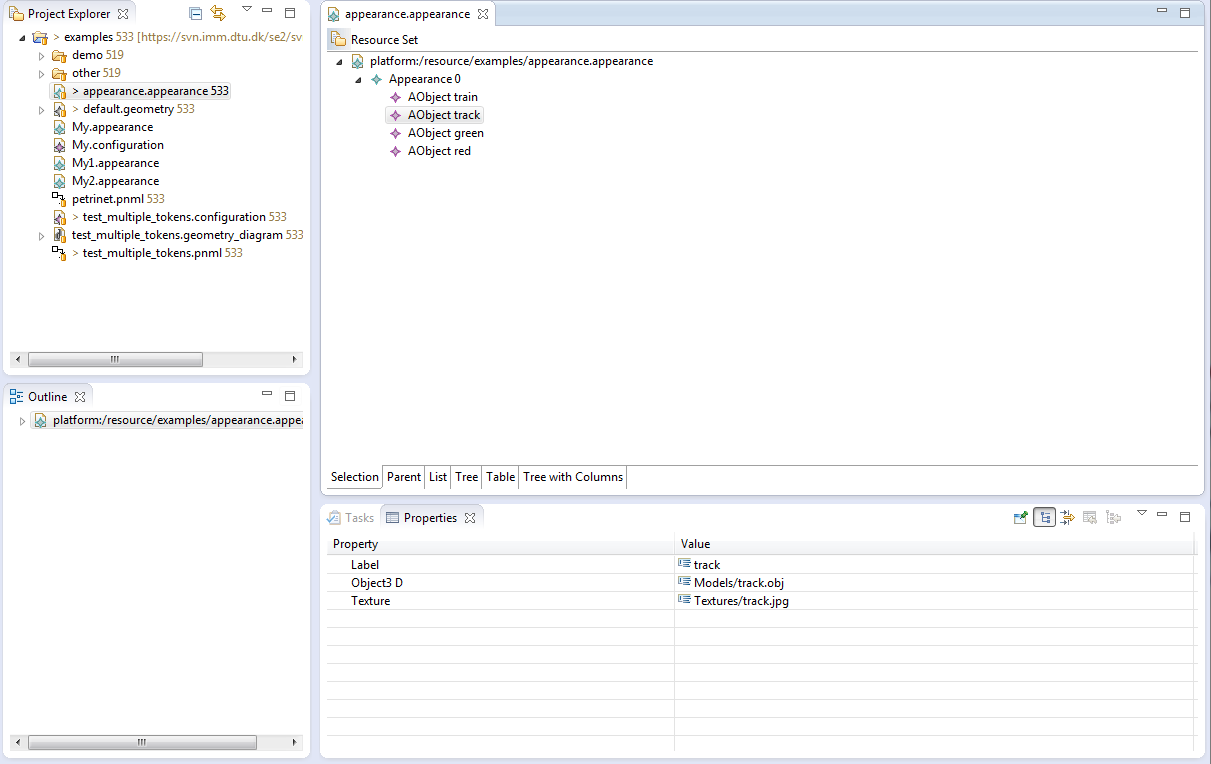
\includegraphics[scale=0.45]{image/ui/appearance.png}
\caption{The Appearance editor GUI.}
\label{fig:appearance_editor}
\end{center}
\end{figure}

\subsubsection{Configuration editor}
The configuration editor (figure \ref{fig:configuration}) helps the user to set up the 3D simulation. In the editor the user has to specify the Petri net, geometry and appearance that he or she wants to use for the 3D simulation. This way the user can for example have different Petri nets but still use the same visual representation for tokens and places in the simulator.

\subsubsection{Simulation tool}
When the user has set up the Configuration successfully he will be able to run the 3D simulation. The 3D simulation opens in a new window. This window has a \textbf{play/pause} button that changes according to the play state; if the simulation state is play the button will be a pause symbol and the other way around. The window also has a \textbf{reset} button that allows the user to reset the simulation.
The user will be able to interact with the simulation, therefore the user will be able to use the mouse to click on different objects. The user will also be able to use the mouse and keyboard to change the camera perspective. An example of the simulation tool can be seen in Figure \ref{fig:simulation_tool}.

\begin{figure}[ht]
\begin{center}
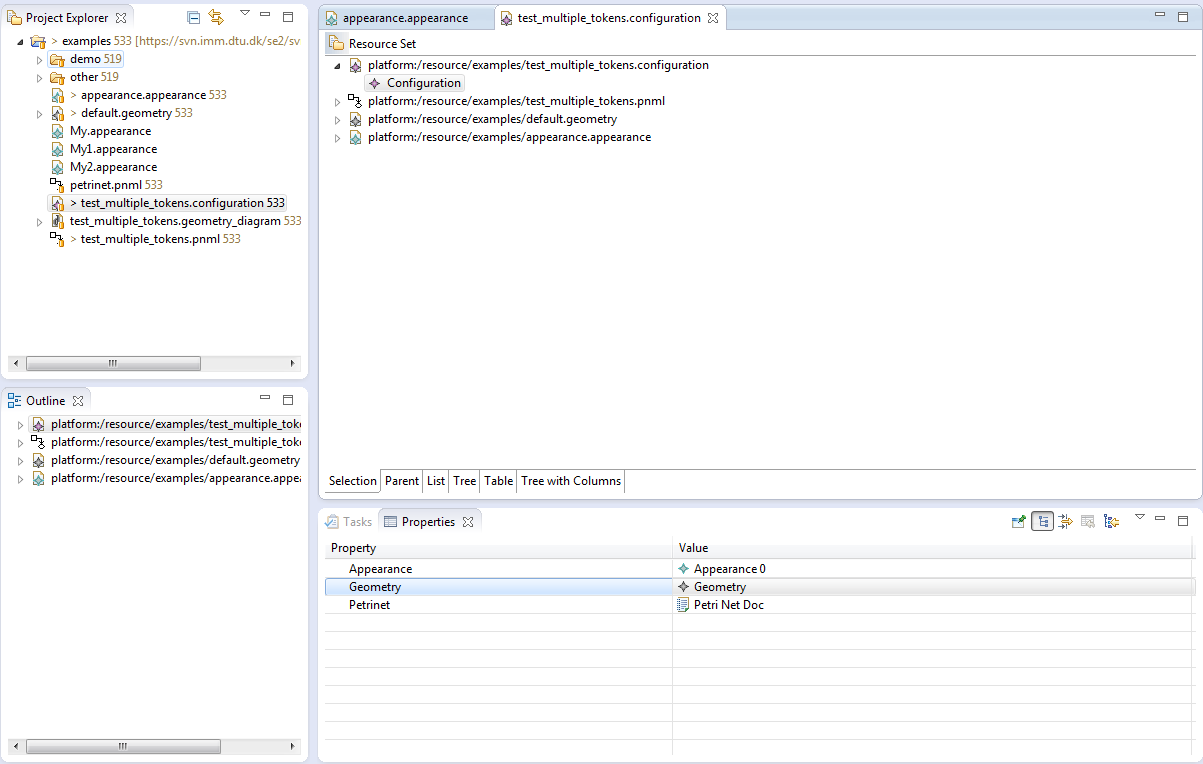
\includegraphics[scale=0.45]{image/ui/configuration.png}
\caption{The configuration editor.}
\label{fig:configuration}
\end{center}
\end{figure}

\begin{figure}[ht]
\begin{center}
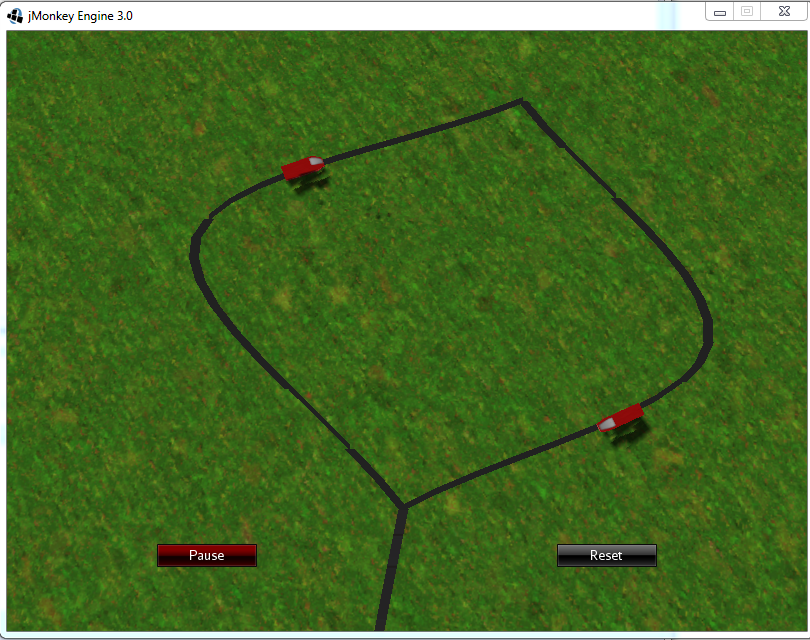
\includegraphics[scale=0.5]{image/ui/simulator.png}
\caption{An example of the Simulation tool.}
\label{fig:simulation_tool}
\end{center}
\end{figure}
